\chapter{Trainers}
A Pokémon GO account is synonymous with its associated Trainer.

\section{Levels\label{sec:levels}}
New Trainers start at Level 1 (of 50) with 0 XP\@.
A new Level is conferred as soon as the Trainer's XP meets or exceeds
  that Level's XP threshold (\autoref{table:xp40}).
It is possible to advance multiple Levels via a single award of XP\@.
\begin{table}
\centering
\begin{tabular}{r r r|r r r}
  Level & kXP & ΔkXP & Level & kXP & ΔkXP \\
\Midrule
1 & 0 & 0 & 21 & 260 & 50 \\
2 & 1 & 1 & 22 & 335 & 75 \\
3 & 3 & 2 & 23 & 435 & 100 \\
4 & 6 & 3 & 24 & 560 & 125 \\
5 & 10 & 4 & 25 & 710 & 150 \\
6 & 15 & 5 & 26 & 900 & 190 \\
7 & 21 & 6 & 27 & 1,100 & 200 \\
8 & 28 & 7 & 28 & 1,350 & 250 \\
9 & 36 & 8 & 29 & 1,650 & 300 \\
10 & 45 & 9 & 30 & 2,000 & 350 \\
11 & 55 & 10 & 31 & 2,500 & 500 \\
12 & 65 & 10 & 32 & 3,000 & 500 \\
13 & 75 & 10 & 33 & 3,750 & 750 \\
14 & 85 & 10 & 34 & 4,750 & 1,000 \\
15 & 100 & 15 & 35 & 6,000 &1,250  \\
16 & 120 & 20 & 36 & 7,500 &7,500  \\
17 & 140 & 20 & 37 & 9,500 &2,000  \\
18 & 160 & 20 & 38 & 12,000&2,500   \\
19 & 185 & 25 & 39 & 15,000&3,000   \\
20 & 210 & 25 & 40 & 20,000&5,000   \\
\end{tabular}
\caption{Requirements for Trainer Levels 1--40\label{table:xp40}}
\end{table}
Levels 41 and above have extra requirements beyond XP (\autoref{table:xp41plus}).
\begin{table}
\centering
  \begin{tabular}{rrrp{0.65\textwidth}}
Level & MXP & ΔMXP & Special requirements \\
\Midrule
41 & 26 & 6 & 20 Legendary/Mythical power ups,\newline
                      30 raid wins, 5 Gold medals,\newline
                      200 Pokémon caught in calendar day\\
42 & 33.5 & 7.5 & Evolve all 8 Eevee forms, 3 excellent throws,\newline
                      200 Pokémon caught with berries,\newline
                      15 item-assisted evolutions\\
43 & 42.5 & 9 & Earn 100k Stardust, 5 platinum medals,\newline
                      200 effective Charged Attacks,\newline
                      5 Legendary/Mythical catches \\
44 & 53.5 & 11 & 30 Trainer Battle wins in each of Great, Ultra, and Master League,
                       20 GO Battle League wins \\
45 & 66.5 & 13 & 100 GO Rocket Grunt wins,
                       100 Pokémon purified,
                       50 GO Rocket Leader wins,
                       10 platinum medals\\
46 & 82 & 15.5 & 100 Field Research tasks,
                       7 consecutive days w/snapshot,
                       50 Excellent throws,
                       30 Eggs hatched\\
47 & 100 & 18 & 30 raid wins with heterogenous teams,\newline
                        3🟉+ Raid win with CP1500-bounded team,\newline
                        3 power ups to Max CP, 20 platinum medals\\
48 & 121 & 21 & 10 Souvenirs from buddy,
                        300 hearts with buddy,
                        200 km walked with buddy,
                        8 weeks with 25 km walked\\
49 & 146 & 25 & 10 trades of 300 km+ catch distance,
                        50 Lucky Pokémon received in trades,
                        500 gifts sent,
                        35 platinum medals\\
50 & 176 & 30 & 5 consecutive Legendary/Mythical catches,
                        3 GO Rocket Leader wins with CP2500-bounded teams,
                        Rank 10 in GO Battle League,
                        999 Excellent throws\\
\end{tabular}
\caption[Requirements for Trainer Levels 41--50]{Requirements for Trainer Levels 41--50.
   Only the medal requirements take prior achievements into account; everything else
   must be accomplished after the challenge has been unlocked.\label{table:xp41plus}}
\end{table}
Certain elements of gameplay are gated by Trainer Level (\autoref{table:levelgates}),
  and a Trainer cannot control Pokémon whose Level exceeds the Trainer's
  by more than 10---a Level 22 Trainer will be unable to power up (\autoref{sec:plevel}) a Pokémon past Level 32.
Reaching a new Level is rewarded with items (\autoref{table:levelitems}).
Levels 7, 8, 13, 15, and 20 introduce Special Research (\autoref{sec:research}), as do
 43, 45, 48, and 50 (under the guise of ``challenges'').
\begin{table}
  \centering
  \begin{tabular}{r p{0.75\textwidth}}
  Level & Features unlocked \\
\Midrule
  2 & Nanab berries \\
  5 & Potions, Revives, Teams, Appraisal, Gyms, Raids \\
  7 & Adventure Incense, ``An Intriguing Incense''\\
  8 & Razz berries, Team GO Rocket, ``A Troubling Situation'' \\
  10 & Super Potions, Golden Razz berries, Evolution items, Trades, Trainer Battles \\
  12 & Great Balls \\
  13 & Max Pokémon and Battles, ``To The Max!''\\
  15 & Hyper Potions, Fast TMs, Parties,\newline``A Mythical Discovery'' \\
  18 & Pinap berries \\
  20 & Silver Pinap berries, Ultra Balls, Mega Evolution,\newline``A Mega Discovery'' \\
  25 & Max Potions, Charged TMs \\
  30 & Max Revives, Route submission \\
  31 & XL Candy \\
  37 & Pokéstop submission \\
\end{tabular}
  \caption{Features unlocked by Trainer Levels\label{table:levelgates}}
\end{table}
\begin{table}
\centering
\setlength{\tabcolsep}{1pt}
\footnotesize
\begin{tabular}{r|g c g c g c g c g c g c g c g c g c g c g c g}
&

\includegraphics[width=1em]{images/pokeball.png} &

\includegraphics[width=1em]{images/greatball.png} &

\includegraphics[width=1em]{images/ultraball.png} &

\includegraphics[width=1em]{images/nanab.png} &

\includegraphics[width=1em]{images/razz.png} &

\includegraphics[width=1em]{images/pinap.png} &

\includegraphics[width=1em]{images/silverpinap.png} &

\includegraphics[width=1em]{images/incense.png} &

\includegraphics[width=1em]{images/revive.png} &

\includegraphics[width=1em]{images/maxrevive.png} &

\includegraphics[width=1em]{images/Potion.png} &

\includegraphics[width=1em]{images/superpotion.png} &

\includegraphics[width=1em]{images/Hyper_Potion.png} &

\includegraphics[width=1em]{images/Max_Potion.png} &
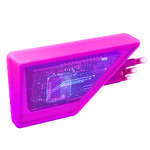
\includegraphics[width=1em]{images/lure.png} &

\includegraphics[width=1em]{images/luckyegg.png} &

\includegraphics[width=1em]{images/rarecandy.png} &

\includegraphics[width=1em]{images/incubatorlimited.png} &

\includegraphics[width=1em]{images/incubatorsuper.png} &

\includegraphics[width=1em]{images/rarecandyxl.png} &

\includegraphics[width=1em]{images/pokecoin.png} &

\includegraphics[width=1em]{images/elitefasttm.png} &

\includegraphics[width=1em]{images/elitechargedtm.png}
  \\
  2 & 10 &    &    &  6 &    &    &    &   &    &    &    &    &    &    &   &   &    &   &   &   &   &   &   \\
  3 & 15 &    &    &  8 &    &    &    &   &    &    &    &    &    &    &   &   &    &   &   &   &   &   &   \\
  4 & 15 &    &    & 15 &    &    &    &   &    &    &    &    &    &    &   &   &    &   &   &   &   &   &   \\
  5 & 20 &    &    &    &    &    &    & 1 & 10 &    & 10 &    &    &    &   &   &    &   &   &   &   &   &   \\
  6 & 15 &    &    &    &    &    &    &   &  5 &    & 10 &    &    &    &   &   &    & 1 &   &   &   &   &   \\
  7 & 15 &    &    &    &    &    &    & 1 &  5 &    & 10 &    &    &    &   &   &    &   &   &   &150&   &   \\
  8 & 15 &    &    &    & 10 &    &    &   &  5 &    & 10 &    &    &    & 1 &   &    &   &   &   &   &   &   \\
  9 & 15 &    &    &    &  3 &    &    &   &  5 &    & 10 &    &    &    &   & 1 &    &   &   &   &   &   &   \\
  10 & 20 &    &    &    & 10 &    &    & 1 & 10 &    &    & 20 &    &    & 1 & 1 &    & 1 &   &   &   &   &   \\
  11 & 15 &    &    &    &  3 &    &    &   &  3 &    &    & 10 &    &    &   &   &    &   &   &   &   &   &   \\
  12 &    & 20 &    &    &  3 &    &    &   &  3 &    &    & 10 &    &    &   &   &    &   &   &   &   &   &   \\
  13 &    & 10 &    &    &  3 &    &    &   &  3 &    &    & 10 &    &    &   &   &    &   &   &   &   &   &   \\
  14 &    & 10 &    &  3 &    &    &    &   &  3 &    &    & 10 &    &    &   &   &    &   &   &   &   &   &   \\
  15 &    & 15 &    &    & 10 &    &    & 1 & 10 &    &    &    & 20 &    & 1 & 1 &    & 1 &   &   &   &   &   \\
  16 &    & 10 &    &  5 &    &    &    &   &  5 &    &    &    & 10 &    &   &   &    &   &   &   &   &   &   \\
  17 &    & 10 &    &    &  5 &    &    &   &  5 &    &    &    & 10 &    &   &   &    &   &   &   &   &   &   \\
  18 &    & 10 &    &    &    &  5 &    &   &  5 &    &    &    & 10 &    &   &   &    &   &   &   &   &   &   \\
  19 &    & 15 &    &    &  5 &    &    &   &  5 &    &    &    & 10 &    &   &   &    &   &   &   &   &   &   \\
  20 &    &    & 20 & 20 &    &    &    & 2 & 20 &    &    &    & 20 &    & 2 & 2 &    & 2 &   &   &   &   &   \\
  21 &    &    & 10 &    &    & 10 &    &   & 10 &    &    &    & 10 &    &   &   &    &   &   &   &   &   &   \\
  22 &    &    & 10 &    & 10 &    &    &   & 10 &    &    &    & 10 &    &   &   &    &   &   &   &   &   &   \\
  23 &    &    & 10 & 10 &    &    &    &   & 10 &    &    &    & 10 &    &   &   &    &   &   &   &   &   &   \\
  24 &    &    & 15 &    & 10 &    &    &   & 10 &    &    &    & 10 &    &   &   &    &   &   &   &   &   &   \\
  25 &    &    & 25 &    &    & 15 &    & 1 & 15 &    &    &    &    & 20 & 1 & 1 &    & 1 &   &   &   &   &   \\
  26 &    &    & 10 &    & 15 &    &    &   & 10 &    &    &    &    & 15 &   &   &    &   &   &   &   &   &   \\
  27 &    &    & 10 & 15 &    &    &    &   & 10 &    &    &    &    & 15 &   &   &    &   &   &   &   &   &   \\
  28 &    &    & 10 &    & 15 &    &    &   & 10 &    &    &    &    & 15 &   &   &    &   &   &   &   &   &   \\
  29 &    &    & 10 &    &    & 15 &    &   & 10 &    &    &    &    & 15 &   &   &    &   &   &   &   &   &   \\
  30 &    &    & 30 &    & 20 &    &    & 3 &    & 20 &    &    &    & 20 & 3 & 3 &    & 3 &   &   &   &   &   \\
  31 &    &    & 10 & 15 &    &    &    &   &    & 10 &    &    &    & 15 &   &   &    &   &   &   &   &   &   \\
  32 &    &    & 10 &    & 15 &    &    &   &    & 10 &    &    &    & 15 &   &   &    &   &   &   &   &   &   \\
  33 &    &    & 10 &    &    & 15 &    &   &    & 10 &    &    &    & 15 &   &   &    &   &   &   &   &   &   \\
  34 &    &    & 10 &    & 15 &    &    &   &    & 10 &    &    &    & 15 &   &   &    &   &   &   &   &   &   \\
  35 &    &    & 30 & 20 &    &    &    & 2 &    & 20 &    &    &    & 20 & 1 & 1 &    & 1 &   &   &   &   &   \\
  36 &    &    & 20 &    & 20 &    &    &   &    & 10 &    &    &    & 20 &   &   &    &   &   &   &   &   &   \\
  37 &    &    & 20 &    &    & 20 &    &   &    & 10 &    &    &    & 20 &   &   &    &   &   &   &   &   &   \\
  38 &    &    & 20 &    & 20 &    &    &   &    & 10 &    &    &    & 20 &   &   &    &   &   &   &   &   &   \\
  39 &    &    & 20 & 20 &    &    &    &   &    & 10 &    &    &    & 20 &   &   &    &   &   &   &   &   &   \\
  40 &    &    & 40 &    & 40 &    &    & 4 &    & 40 &    &    &    & 40 & 4 & 4 &    & 4 &   &   &   &   &   \\
  41 &    &    & 20 &    & 20 &    &    &   &    & 20 &    &    &    & 20 &   &   & 1  & 1 &   & 1 &   &   &   \\
  42 &    &    & 20 & 20 &    &    &    &   &    & 20 &    &    &    & 20 &   &   & 1  & 1 &   & 1 &   &   &   \\
  43 &    &    & 20 &    &    &    & 20 &   &    & 20 &    &    &    & 20 &   &   & 1  & 1 &   & 1 &   &   &   \\
  44 &    &    & 20 &    & 20 &    &    &   &    & 20 &    &    &    & 20 &   &   & 1  & 1 &   & 1 &   &   &   \\
  45 &    &    & 40 &    &    &    &    & 2 &    & 40 &    &    &    &    & 2 & 2 & 1  &   & 1 & 2 &   & 1 &   \\
  46 &    &    & 30 &    & 25 &    &    &   &    & 20 &    &    &    & 25 &   &   & 1  & 1 &   & 1 &   &   &   \\
  47 &    &    & 30 & 25 &    &    &    &   &    & 20 &    &    &    & 25 &   &   & 1  & 1 &   & 1 &   &   &   \\
  48 &    &    & 30 &    &    &    & 15 &   &    & 20 &    &    &    & 25 &   &   & 1  & 1 &   & 1 &   &   &   \\
  49 &    &    & 30 &    &    & 25 &    &   &    & 20 &    &    &    & 25 &   &   & 1  & 1 &   & 1 &   &   &   \\
  50 &    &    & 50 &    &    &    &    & 5 &    &    &    &    &    & 50 & 5 & 5 & 2  &   & 5 & 2 &   &   & 1 \\
\end{tabular}
\caption{Items awarded for reaching Trainer Levels\label{table:levelitems}}
\end{table}
All level-gated mechanics, including the ability to fully power up Pokémon,
 are available at Level 40\footnote{The maximum Pokémon Level is 50 (\autoref{chap:pokemon}).}.
Levels 41, 43, 45, 47, 49, and 50 open some cosmetic options for Trainer avatars.
Trainer Level determines the maximum level of wild spawns
  (\autoref{sec:spawns}) and the difficulty of Team GO Rocket
  opponents (\autoref{subsec:rocket}).

\section{Team}
Upon reaching Level 5, a Trainer can join one of three Teams: Mystic (blue),
  Valor (red), or Instinct (yellow).
The only non-cosmetic effect of Team choice regards gyms (\autoref{sec:gyms}), which
  are held by one Team at a time.
A Trainer can change their Team by purchasing and making use of a Team Medallion.
The cost is 1,000 Pokécoins, and 365 days must pass between Medallion purchases.

It seems sadly impossible to join GO Rocket. Alas!

\section{Capacities and initial inventories\label{sec:capacities}}
Trainers enter this world with no Pokémon, no Pokécoins, no Stardust,
  no Max Particles, no Candy of any kind, no Mega Energy of any kind,
  no Primal Energy of any kind, no Fusion Energy of any kind, and no Crown
  Energy of any kind.
They have initial carrying capacity sufficient for 300 Pokémon.
Additional storage can be added in increments of 50, up to a total of 10,500.
Each upgrade costs 200 Pokécoins.
A full upgrade will thus currently run you 40,800 Pokécoins.

During the initial tour with Professor Willow, the Trainer selects one of
 Bulbasaur, Charmander, Squirtle, or Pikachu to catch.
They will enter the Encounter screen, be provided an infinite supply of
  Pokéballs for the encounter, and enjoy a catch rate (\autoref{sec:catch}) set to 100\%.

The Trainer has a Bag capable of storing 350 items (strangely, not all items
  count against this limit, including Gifts, Stickers, and the Postcard Book,
  which I suppose are shoved down the front of one's Trainer uniform).
The Bag comes with an Infinite Incubator, a Camera, 2 Incense, and 50 Poké Balls,
  and thus space for 296 new items.
The Bag can be upgraded to store up to 9,500 items.
Here again, each upgrade costs 200 Pokécoins, and increases capacity by 50 items.
The maximum Bag is thus 36,600 Pokécoins.

The Trainer has a Postcard Book with seven pages, each capable of retaining
 50 Postcards, for an initial limit of 350.
Pages can be added for 100 Pokécoins each, up to a maximum of 40 Pages
 supporting 2,000 total Postcards.
Such a monster will cost 3,300 Pokécoins.

The Trainer can carry up to twenty Gifts at a time, and up to 25 of each sticker.
To date, no one has found any use for the stickers.

Upon obtaining four Shadow Shards, they are automatically refined into a Purified Gem.
The Trainer can carry up to ten Purified Gems.
Shadow Shards cannot be collected while holding ten gems, though any extras
 following the tenth gem's purification will be retained (this can only
 happen when receiving multiple shards in a single award).

A trainer cannot collect Max Particles while in possession of 1,500 or more.
The Trainer can collect no more than 9,999 units of any Mega Energy,
 Primal Energy, or Fusion Energy.
A limit on Crown Energy is not yet known, but seems likely to be 9,999.

No limit is known for Candy nor Candy XL\@.
A lower bound has been established in the millions.
It seems plausible that the limit is one less than a large power of 2:
  2,147,483,647 seems as good a guess as any\footnote{If the limit is driven by UI requirements, it's likely lower.}.

Trainers will not infrequently receive rewards which, combined with existing supplies, exceed capacity.
The full award will be processed in such cases.
If capacity has been met or exceeded before the award, however, no part of the award is received.
Since Pokémon are never acquired other than one at a time, this situation cannot
 arise for them.
When Pokémon storage is full, the Trainer will not be allowed to incubate eggs,
 nor enter encounters.
They can fight raids etc., but the bonus challenge will be skipped.
Having upgraded storage or otherwise made space available, the Trainer can
 reenter and complete the challenge (assuming the relevant raid boss/Power Stop is
 still available).

\section{Pokédexen\label{sec:dexen}}
The Trainer has ten Pokédexen\footnote{``Pokédexes'' to the uncultured.}:
  ``Pokémon'', ``Shiny'', ``XXL'', ``XXS'', ``G-Max'', ``Mega'', ``Shadow'',
  ``Purified'', ``🟉100\%'', and ``Lucky''.
All ten start empty, and several start locked.
Unlocking ``🟉100\%'' requires 20 4🟉 Pokémon.
15 Shiny Pokémon must be captured for ``Shiny''.
10 Shadow, Purified, or Lucky Pokémon will unlock their respective dexen.
Entries are filled in as the relevant Pokémon are acquired (via any means).
Once registered, Pokédex entries are never unregistered.
If an entry is made in some Pokédex, the corresponding entry is also made
  in the primary Pokédex.
Shiny Shadow Pokémon and Shiny Purified Pokémon are registered to the
  ``Shiny'' Pokédex along with the ``Shadow'' or ``Purified'' Pokédex.
Effective searching is covered in \autoref{sec:searching}.

Besides pointless nostalgia, the ``Info'' and ``Battle'' tabs of filled entries
  provide information regarding evolution (\autoref{sec:evolution}), type
  relations (\autoref{chap:types}), and attacks (\autoref{chap:attacks}).
Trainers can place an alert on one filled or silhouetted entry to receive
  notifications when that Pokémon is nearby.

\begin{tipbox}[title=Living Pokédexen]
Some extreme collectors maintain ``living Pokédexen'', i.e.\ one of each
  species/form in their usable Pokémon storage.
I suppose you never know when you'll need reach for Emolga.
\end{tipbox}

\section{Grinding\label{sec:grinding}}
For me, the joy of Pokémon GO is almost entirely found in its PvP League play (\autoref{sec:3x3}).
Others take pleasure from its collection and social aspects.
Either way, you'll be doing a good bit of slogging in order to find, develop,
  and evolve powerful Pokémon.
Those willing to spend money can speed the process up a bit, but there's
  no escaping the fundamental cycles of Catch, Appraise, Transfer and
  Catch, Appraise, Develop. 
I began playing on 2025-03-01.
As I write this about four months later, I have caught 26,539 Pokémon, and retained 441---a little less than 1.7\%.

\subsection{Grinding Pokémon\label{subsec:getmons}}
Pokémon can be received via trades (\autoref{sec:trades}),
  and hatched from eggs (\autoref{sec:eggs}),
  but most are caught with Pokéballs in encounters.
An encounter involves a single subject Pokémon, a single Trainer,
  and possibly that Trainer's current Buddy Pokémon.
Outcomes (aside from certain plot-based encounters) include capture, flight, and departure.

Pokémon will spawn on the Map screen, seemingly at random (see \autoref{sec:spawns} for details).
Pressing on them will open the Encounter screen with that Pokémon,
  providing an opportunity to catch it.
Encounters are also triggered by the completion of certain Research,
  defeats of Team GO Rocket, Raid wins, and Max Battle wins.
Up to one hundred encounters from Research can be arbitrarily postponed by leaving the encounter,
  or simply not closing the research out.
Leaving wild encounters might see the Pokémon disappear from the Map, especially
  if you've moved significantly, or much time has gone by.
Victories against Team GO Rocket in their balloon are a one-and-done deal:
  the balloon will depart if the Trainer exits the encounter.

\subsection{Grinding XP\label{subsec:getxp}}
Gaining sufficient XP advances the Trainer's level.
It is most regularly received for capturing Pokémon, but large awards are
  available by other means, and can be the source of a majority of a Trainer's XP.
The Gifts system is essentially a machine for converting
  time into experience points (\autoref{sec:gifts}).
Raids and Max Battles, especially 4🟉 or higher, are munificent with the XP.
Using a Lucky Egg doubles all XP awards for thirty minutes (time remaining is displayed on the upper right of the map).
Lucky Eggs can be bought from the Shop (one for 80 Pokécoins or eight for 500),
  and are sometimes awarded for completing Research.
Routes and showcases can also be good sources of XP\footnote{My recent rather dubious 159th place in a Zacian showcase netted 1000 XP\@.}.

\begin{table}
\centering
\begin{tabular}{lr}
Action & XP\\
\Midrule
  Feed berry to Gym defender & 50\\
  Spin Pokéstop & 50\\
  Sending a Gift & 200\\
  Spin new Pokéstop & 250\\
  New main Pokédex registration & 1000\\
  Pokémon evolution & 1000\\
  Research breakthrough & 3000\\
\end{tabular}
\caption{XP awards not captured elsewhere\label{table:xpawards}}
\end{table}

\subsection{Grinding Stardust\label{subsec:getdust}}
Trainers pay a cost (partially) in Stardust
  to level up their Pokémon (\autoref{sec:plevel}),
  to trade them (\autoref{sec:trades}),
  to purify Shadow Pokémon (\autoref{sec:shadow}),
  to teach them second charged attacks (\autoref{sec:charged}),
  to change certain forms (\autoref{sec:forms}),
  and to activate Adventure Effects (\autoref{sec:effects}).
Stardust becomes the primary bottleneck on advancement fairly early in the game:
  Pokémon at higher levels require more Stardust to power up (\autoref{table:powerups}),
  but the amount of Stardust awarded for their capture doesn't change.
There is never enough.

The primary means of acquiring Stardust is catching Pokémon.
The vast majority of Pokémon result in one of three awards based on their stage
 (\autoref{sec:evolution}), but a few offer more (\autoref{table:stardust}),
 making them excellent targets for Razz berries.
A Pokémon which is weather-boosted (\autoref{sec:weather}) awards 25\% more than normal.
Stardust can also be collected for wins in the GO Battle League,
  opening Gifts (\autoref{sec:gifts}),
  completing Routes,
  completing Research,
  participating in Showcases,
  defeating Team Leaders in Trainer Battles,
  defeating Team GO Rocket,
  hatching eggs,
  feeding berries to Pokémon defending your team's gyms (30 per),
  and from weekly Adventure Sync rewards based on the total distance walked.
5🟉 and 6🟉 Max Battles award 15,000 and 25,000 Stardust respectively.
A Star Piece increases all Stardust awards by 50\% for thirty minutes.
Star Pieces can be bought from the Shop (individually, or eight at wholesale), and are sometimes awarded for Research.
\begin{table}
\centering
\begin{tabular}{p{.7\textwidth}rr}
Pokémon & Award & w/boost\\
\Midrule
Audino & 2100 & 2625\\
Cloyster & 1200 & 1500\\
Shellder, Chimecho & 1000 & 1250\\
Alolan Persian, Starmie, Vespiquen, Garbodor & 950 & 1188\\
Alolan Meowth, Staryu, Sableye, Combee,\newline
\hspace{\parindent}Trubbish & 750 & 938\\
Parasect, Persian, Breloom, Amoonguss, Shiinotic & 700 & 875\\
Paras, Meowth, Delibird, Shroomish, Foongus,\newline
\hspace{\parindent}Morelull, and stage 3 Pokémon not yet specified & 500 & 625\\
Stage 2 Pokémon not yet specified & 300 & 375\\
All other Pokémon & 100 & 125\\
\end{tabular}
\caption{Stardust awards for capturing Pokémon\label{table:stardust}}
\end{table}
\subsection{Grinding Candy\label{subsec:getcandy}}
Each genus (\autoref{sec:evolution}) has its own flavor of Candy and Candy XL\@.
Along with Stardust, most Pokémon enhancement is driven by Candy.
Candy is primarily acquired by capturing Pokémon: each capture (in any context)
  awards Candy (and possibly Candy XL) of the capture's genus.
Three Candy are awarded for capture of a Stage 1 Pokémon, five for a Stage 2,
  and ten for Stage 3\footnote{Legendaries give only three, even if they're evolved.}.
Pinap and Silver pinap berries increase this award (\autoref{sec:berries}).
Candy XL is necessary for advancing Pokémon past level 40.
100 Candy can be exchanged for a single Candy XL of that flavor.
Each Rare Candy can be converted into arbitrarily flavored Candy; Rare Candy XL can become any flavor of Candy XL\@.

A Pokémon can be ``transferred to the Professor'' for soul harvesting.
Its loss of existence is your gain of one tasty Candy.
Certain plot armored Pokémon cannot be harvested (\autoref{sec:regions}).
Pokémon can be transferred to a linked Pokémon HOME account, resulting in a single Candy.
Evolution consumes many Candies, but returns one when complete.
Trading (\autoref{sec:trades}) nets Candy (and possibly Candy XL) of the Pokémon traded away.
Winning Max Battles awards Candy (and possibly Candy XL);
 5🟉 and 6🟉 Max Battles award 10 and 30 Candy.

Walking with a Buddy (\autoref{sec:buddies}) will generate Candy (and possibly Candy XL and Mega Energy).
The distance that must be walked depends on the Buddy's cost group (\autoref{sec:costgroups}),
 and whether the Buddy is ``active'' (on the map).
Giving berries to gym defenders rarely results in Candy (in addition to guaranteed XP and Stardust).
Hatching an egg yields substantial Candy of the hatched genus, depending on the egg type (\autoref{sec:eggs}).
It is possible through Research to receive Candy for a genus not present in
  your Pokédex, i.e.\ one whose constituent species you have never captured.
You'll keep this Candy, but it doesn't result in a Pokédex entry.
Likewise, Candy is retained even if all Pokémon of that genus have been transferred.
\subsection{Grinding particles}
Interacting with Power Stops awards Max Particles once per day per Stop.
Each Stop awards 120 the first time, and 100 subsequently.
Walking 2km makes available 300 MP\@.
Claiming them resets the pedometer, which does not track walking while they're unclaimed.
Once 800 or more MP have been collected on a calendar day via these methods, no
 more can be collected\footnote{Note that this allows up to 1080 MP per day.
 Claim a walk award and interact with four new Power Stops for 780 MP, then
 close it out with a walk award.}.
This timer resets at 0500h local time.
Max Particles from Research are not subject to this restriction, nor are Max Particle Packs.
Available from the Shop (individually, or in packs of three), each contains 800 MP\@.

\subsection{Grinding energies}
Form-changing energies (Mega, Primal, Fusion, and Crown) can be acquired by
 winning a raid of that type or completing certain research tasks.
The amount of Mega or Primal energy awarded depends on how quickly the raid is won.
If a Buddy Pokémon is of an evolutionary line where any member of that line has undergone Mega evolution
  or Primal reversion, walking will earn 5 energy per kilometer.
This rate is constant across all species, but the energy is awarded only when the Buddy finds Candy,
  as determined by its cost group (\autoref{sec:costgroups}).
Walking cannot earn Fusion or Crown energies.
Very rarely, spinning Pokéstops will result in Beedrill Mega energy.

Note that Mega and Primal evolutions are temporary, while Fusion and Crowning is persistent
  until explicitly undone.
\subsection{Grinding Pokécoins (and F2P vs. P2P)\label{subsec:getcoins}}
Pokémon GO is free to download, with optional microtransactions through the in-game
  Shop and the Pokémon GO web store.
Pokécoins can be used to purchase most items\footnote{Event passes generally require cash,
  as does anything specific to the web store.}, and local currency can purchase Pokécoins.
Interestingly, the ratio of exchange rates for Pokécoin and USD diverges
  wildly across regions\footnote{Use of e.g.\ a VPN to purchase Pokécoins remotely is a violation of the ToS\@.}.
A one-time award of 150 Pokécoins (a humble sum ensuring that Trainers are aware of the game's spending opportunities)
  is presented upon reaching Level 7.
More usefully, Pokémon defeated while defending a gym (\autoref{sec:gyms}) can
  return with Pokécoins.
The Pokémon receives one Pokécoin for every ten minutes spent in the Gym, and presents these weregild to the Trainer.
The Trainer can collect only 50 Pokécoin each calendar day (requiring 8⅓ hours' occupancy), no matter how many Pokémon return.

As an example, a Trainer leaves Pokémon in aligned gyms at 2200h and 2210h local time.
The first returns at 2341h that evening, the second at 1001h the next morning.
The Trainer receives 10 Pokécoins at 2341h, and 50 Pokécoins at 1001h, for a total of 60.
If the first returned instead at 0001h, the Trainer would receive 12 Pokécoins at 0001h,
  and 38 Pokécoins at 1001h, for a total of 50.
Note that the second case earns less, despite greater occupancy time.
By regularly taking gyms, with a little luck a Trainer can accumulate 350 free Pokécoins each week.

Is it possible to play PGO at a high level without spending money?
The serious collector-style Trainer has costs for storage and raiding (\autoref{sec:raids})
  that can't easily be met by 350 Pokécoins per week, especially
  in pursuit of Shiny Pokémon (\autoref{sec:shiny}),
  but millions of people collect at a hobbyist level for free.
For the PvP-oriented Trainer, there's little need to spend at all,
  especially if you live in an area with lots of PGO activity.
I have minimal Bag and Pokémon storage (800 and 500 respectively), and raid almost exclusively locally using the daily free pass.
Very few of my Pokémon have the optimal IVs for their Leagues (\autoref{chap:bounded}),
  and I don't yet have many of the Pokémon with which I'd like to experiment,
  yet my Great and Ultra League Elos rarely dip below 2100.
Frankly, I consider my free play a point of pride\footnote{I've spent a little less than 80 USD to date, so not quite ``free''.}.
Whether one needs spend money in Pokémon GO is entirely a matter of goals, dedication, and patience.
With that said, if you want to spend, go with God---thanks for making my free play possible.

The calculus changes for rural Trainers.
Without local raiding (and at least four or five other Trainers to join on larger battles),
  it will be difficult to collect a diverse team of competitive Pokémon.
There are three alternatives: trading (which requires meeting Trainers already in possession of the desired Pokémon;
  see \autoref{sec:trades}), hosting raids, and remote raiding.
Raids can be effectively hosted using the Campfire app or various websites.
Remote raiding requires passes, which require Pokécoins---525 for 3 passes at this time.
Collecting the maximum 50 from gyms eleven out of every fourteen days, you can do
  three free remote raids every two weeks.
You will initially be at a definite disadvantage in PvP, but it is one that can
  be largely overcome with cunning, and eliminated with a year's tenacious
  and savvy play.

\subsection{Grinding items\label{subsec:grinditems}}
A calendar day's first spin of a gym disc wins a raid pass unless one is already held (\autoref{sec:raids}).
Basic berries, low-grade potions, and balls are the constant output of spun Pokéstops.
Gym discs tend to output more potions and revives.
On rare occasions, spins can output evolution items (\autoref{table:itemevolutions}).
Opening a gift can yield items and Stardust.
A sack of items is presented following victories in Team GO Rocket encounters, raids, and Max battles.
Each week, awards are made based on total walking distance.
Each day's first victory against a Team Leader in a Trainer Battle can award items,
  including evolution catalysts.

The most important items to carry are Pokeballs.
Berries are of little use without them\footnote{It's trivial to show successful
 captures consume at least as many balls as berries, and usually more.}.
Encounters are much more frequent than battles; battle rewards almost always
 include potions and revives sufficient to cover damage suffered therein.
I never carry more than about twenty Max Potions and Max Revives, yet keep my Pokémon fully healed at all times.
Once Golden Razz berries are unlocked, there's no point in carrying Razz berries;
  use them immediately in encounters, or feed them to gym defenders.
Nanab berries are only marginally useful (primarily with Shadow Pokémon): eschew them.
Pinap berries are great.
I set out with about half as many Pinaps as balls, and let them fly almost by default.
Rare Silver Pinaps are worth hanging onto for considered use.
Berries ought feed Pokémon, not fill up your bag.

Rare Candy is great when you make active use of it, but more than a hundred
  probably means you've got some underachieving Pokémon.
Rare Candy XL is worth carrying around until you have a Pokémon you really
  want to push above level 40, or whose Max Moves you want at level 3.
More than five of any evolution item seems a bit much.
Elite TMs are precious, but regular TMs (both fast and charged) can be readily
  had from routes.

Even with the default capacities, this discipline ought leave space for at least one hundred balls.
Storage constantly under pressure is not sustainable; I try to keep at least one third free.

\section{Research\label{sec:research}}
Research is a diverse set of challenges, each with its own reward.
The Research screen is summoned up with the binoculars logo in the lower right of the Map screen.
It is broken into three tabs:
\begin{itemize}
  \item \textbf{Events:} Research and bonuses related to the calendar year, including ticketed research.
  \item \textbf{Today:} Field research---short-term (usually) tasks acquired by spinning Pokéstops.
            Field research tasks can be dismissed without completion.
            Up to four field research tasks can be active at a time.
  \item \textbf{Special:} Longer-term research structuring the game's plot, so far as one exists.
    Tasks and rewards are of greater magnitude.
    Special research comes in multipart stories, where each part consists of multiple tasks.
    All tasks within a part must be completed to advance within the story.
\end{itemize}
The rewards of field research are generally on the order of Pokéstop items---berries, balls,
 etc.---but also include encounters.
Special and Event research rewards can be quite substantial, and are the only way to acquire some Pokémon.
Pokémon met in research encounters have a higher IV floor than most spawns (\autoref{table:ivfloors}),
  and are thus disproportionately powerful for their species.
Event research includes Collection Challenges, which require the capture of a set of Pokémon
  within a time period, and are associated with their own medal.

\section{Medals\label{sec:medals}}
A large set of Medals can be achieved at the Bronze, Silver, Gold, or Platinum level (\autoref{table:medals}).
The vast majority are functionally useless, though several levels beyond 40 require earning
  Platinum medals (\autoref{table:xp41plus}).
The ``Hero'' and ``Purifier'' medals result in additional Premier Balls (\autoref{sec:catch})
  when rescuing Shadow Pokémon---1, 2, 3, or 4 extra balls for each tier of each medal.
Medals associated with catching Pokémon of a type give capture rate bonuses of 10\%, 20\%, 30\%, and 40\%.
Catching a dualtyped Pokémon advances both associated medals.
When encountering a dualtyped Pokémon, the catch bonus is averaged between the two relevant medals.
Bronze requires 10 catches, silver 50, gold 200, and platinum 2,500.
The ``Elite Collector'' medal is inscribed with the number of Collection
  Challenges completed (\autoref{sec:research}), and is always gold.
Each region (\autoref{sec:regions}) has an associated medal (\autoref{table:regionmedals}) for filling
  in its primary Pokédex (\autoref{sec:dexen}).
For Vivillon medal details, see \autoref{subsec:vivillon}.
There are a great many event-specific medals; I shan't cover them here.
\begin{table}[t]
\centering
\footnotesize
\begin{tabular}{lrrrr}
  Region & Bronze & Silver & Gold & Platinum\\
  \Midrule
  Kanto & 5 & 50 & 100 & 151\\
  Johto & 5 & 30 & 70 & 100\\
  Hoenn & 5 & 40 & 90 & 135\\
  Sinnoh & 5 & 30 & 80 & 107\\
  Unova & 5 & 50 & 100 & 156\\
  Kalos & 5 & 25 & 50 & 72\\
  Alola & 5 & 25 & 50 & 86\\
  Galar & 5 & 25 & 50 & 89\\
  Hisui & 1 & 3 & 5 & 7\\
  Paldea & 5 & 30 & 80 & 103\\
\end{tabular}
  \caption{Regional Pokédex medals\label{table:regionmedals}}
\end{table}
\begin{table}[t]
\centering
\begin{tabular}{lc|lc|lc}
  Medal & Type & Medal & Type & Medal & Type\\
  \Midrule
  Bug Catcher & 
\includegraphics[width=1em,keepaspectratio]{images/bug.png} &
   Kindler & 
\includegraphics[width=1em,keepaspectratio]{images/fire.png} &
   Schoolkid &
\includegraphics[width=1em,keepaspectratio]{images/normal.png} \\
  Delinquent & 
\includegraphics[width=1em,keepaspectratio]{images/dark.png} &
   Bird Keeper & 
\includegraphics[width=1em,keepaspectratio]{images/flying.png} &
   Punk Girl & 
\includegraphics[width=1em,keepaspectratio]{images/poison.png} \\
  Dragon Tamer & 
\includegraphics[width=1em,keepaspectratio]{images/dragon.png} &
   Hex Maniac &
\includegraphics[width=1em,keepaspectratio]{images/ghost.png} &
   Psychic &
\includegraphics[width=1em,keepaspectratio]{images/psychic.png} \\
  Rocker & 
\includegraphics[width=1em,keepaspectratio]{images/electric.png} &
   Gardener &
\includegraphics[width=1em,keepaspectratio]{images/grass.png} &
   Hiker &
\includegraphics[width=1em,keepaspectratio]{images/rock.png} \\
  Fairy-Tale Girl &
\includegraphics[width=1em,keepaspectratio]{images/fairy.png} &
   Ruin Maniac &
\includegraphics[width=1em,keepaspectratio]{images/ground.png} &
   Rail Staff &
\includegraphics[width=1em,keepaspectratio]{images/steel.png} \\
  Black Belt & 
\includegraphics[width=1em,keepaspectratio]{images/fighting.png} &
   Skier & 
\includegraphics[width=1em,keepaspectratio]{images/ice.png} &
   Swimmer &
\includegraphics[width=1em,keepaspectratio]{images/water.png}\\
\end{tabular}
  \caption{Medals with catch bonuses\label{table:medalcatch}}
\end{table}
\clearpage
\begingroup
\setlength{\tabcolsep}{1pt}
\footnotesize
\begin{longtable}{m{.3\textwidth}m{.4\textwidth}rrrr}
Name & Counts & B & S & G & P\\
\Midrule\endhead
Jogger & km walked & 10 & 100 & 1k & 10k\\
Collector & Captures & 30 & 500 & 2k & 50k\\
Scientist & Evolutions & 3 & 20 & 200 & 2k\\
Breeder & Hatches & 10 & 100 & 500 & 2.5k\\
Backpacker & Pokéstop spins & 100 & 1k & 2k & 50k\\
Sightseer & Unique Pokéstops & 10 & 100 & 1k & 2k\\
Fisher & Large Magikarp captures & 3 & 50 & 300 & 1k\\
Battle Girl & Gym battle wins & 10 & 100 & 1k & 4k\\
Ace Trainer & Team Leader wins & 10 & 100 & 1k & 2k\\
Youngster & Tiny Rattate captures & 3 & 50 & 300 & 1k\\
Pikachu Fan & Pikachu captures & 3 & 50 & 300 & 1k\\
Unown & Unique Unown captures & 3 & 10 & 26 & 28\\
Champion & 4🟉- raid wins & 10 & 100 & 1k & 2k\\
Battle Legend & 5🟉+ raid wins & 10 & 100 & 1k & 2k\\
Berry Master & Gym berry feeds & 10 & 100 & 1k & 15k\\
Gym Leader & Gym occupancy hours & 10 & 100 & 1k & 15k\\
Pokémon Ranger & Field Research & 10 & 100 & 1k & 2.5k\\
Idol & Best Friends & 1 & 2 & 3 & 20\\
Gentleman & Trades & 10 & 100 & 1k & 2.5k\\
Pilot & km of Trades & 1k & 100k & 1M & 10M\\
Great League Veteran & GL wins & 5 & 50 & 200 & 1k\\
Ultra League Veteran & UL wins & 5 & 50 & 200 & 1k\\
Master League\newline{}Veteran & ML wins & 5 & 50 & 200 & 1k\\
Cameraman & Snapshot photobombs & 10 & 50 & 200 & 400\\
Purifier & Purifications & 5 & 50 & 500 & 1k\\
Hero & GO Rocket Grunt\newline{}and Leader wins & 10 & 100 & 1k & 2k\\
Ultra Hero & Giovanni wins & 1 & 5 & 20 & 50\\
Best Buddy & Best Buddies & 1 & 10 & 100 & 200\\
Wayfarer & Wayfarer agreements & 50 & 500 & 1k & 1.5k\\
Triathlete & 7-day streaks & 1 & 10 & 50 & 100\\
Rising Star & Unique raid wins & 2 & 10 & 50 & 150\\
Rising Star Duo & Raid wins w/friends & 10 & 100 & 1k & 2k\\
Picnicker & Pokémon spawned due your Lures, captured by other Trainers & 5 & 25 & 500 & 2.5k\\
Successor & Mega evolutions & 1 & 50 & 500 & 1k\\
Mega Evolution Guru & Unique Mega evolutions & 1 & 24 & 36 & 46\\
Friend Finder & Referred Trainers & 1 & 10 & 20 & 50\\
Raid Expert & Raid Achievements earned & 1 & 50 & 200 & 500\\
Tiny Pokémon\newline{}Collector & XXS height captures & 5 & 25 & 100 & 500\\
Jumbo Pokémon\newline{}Collector & XXL height captures & 5 & 25 & 100 & 500\\
Vivillon Collector & Vivillon medals unlocked & 1 & 5 & 10 & 18\\
Expert Navigator & Routes completed & 10 & 50 & 200 & 600\\
Showcase Star & Showcase contests won & 1 & 10 & 50 & 100\\
Community Member & Campfire event checkins & 1 & 20 & 50 & 100\\
Life of the Party & Party challenges completed & 10 & 50 & 100 & 200\\
  \caption{Unstructured medals\label{table:medals}}
\end{longtable}
\endgroup
